\documentclass[tikz,border=2mm]{standalone}

\begin{document}
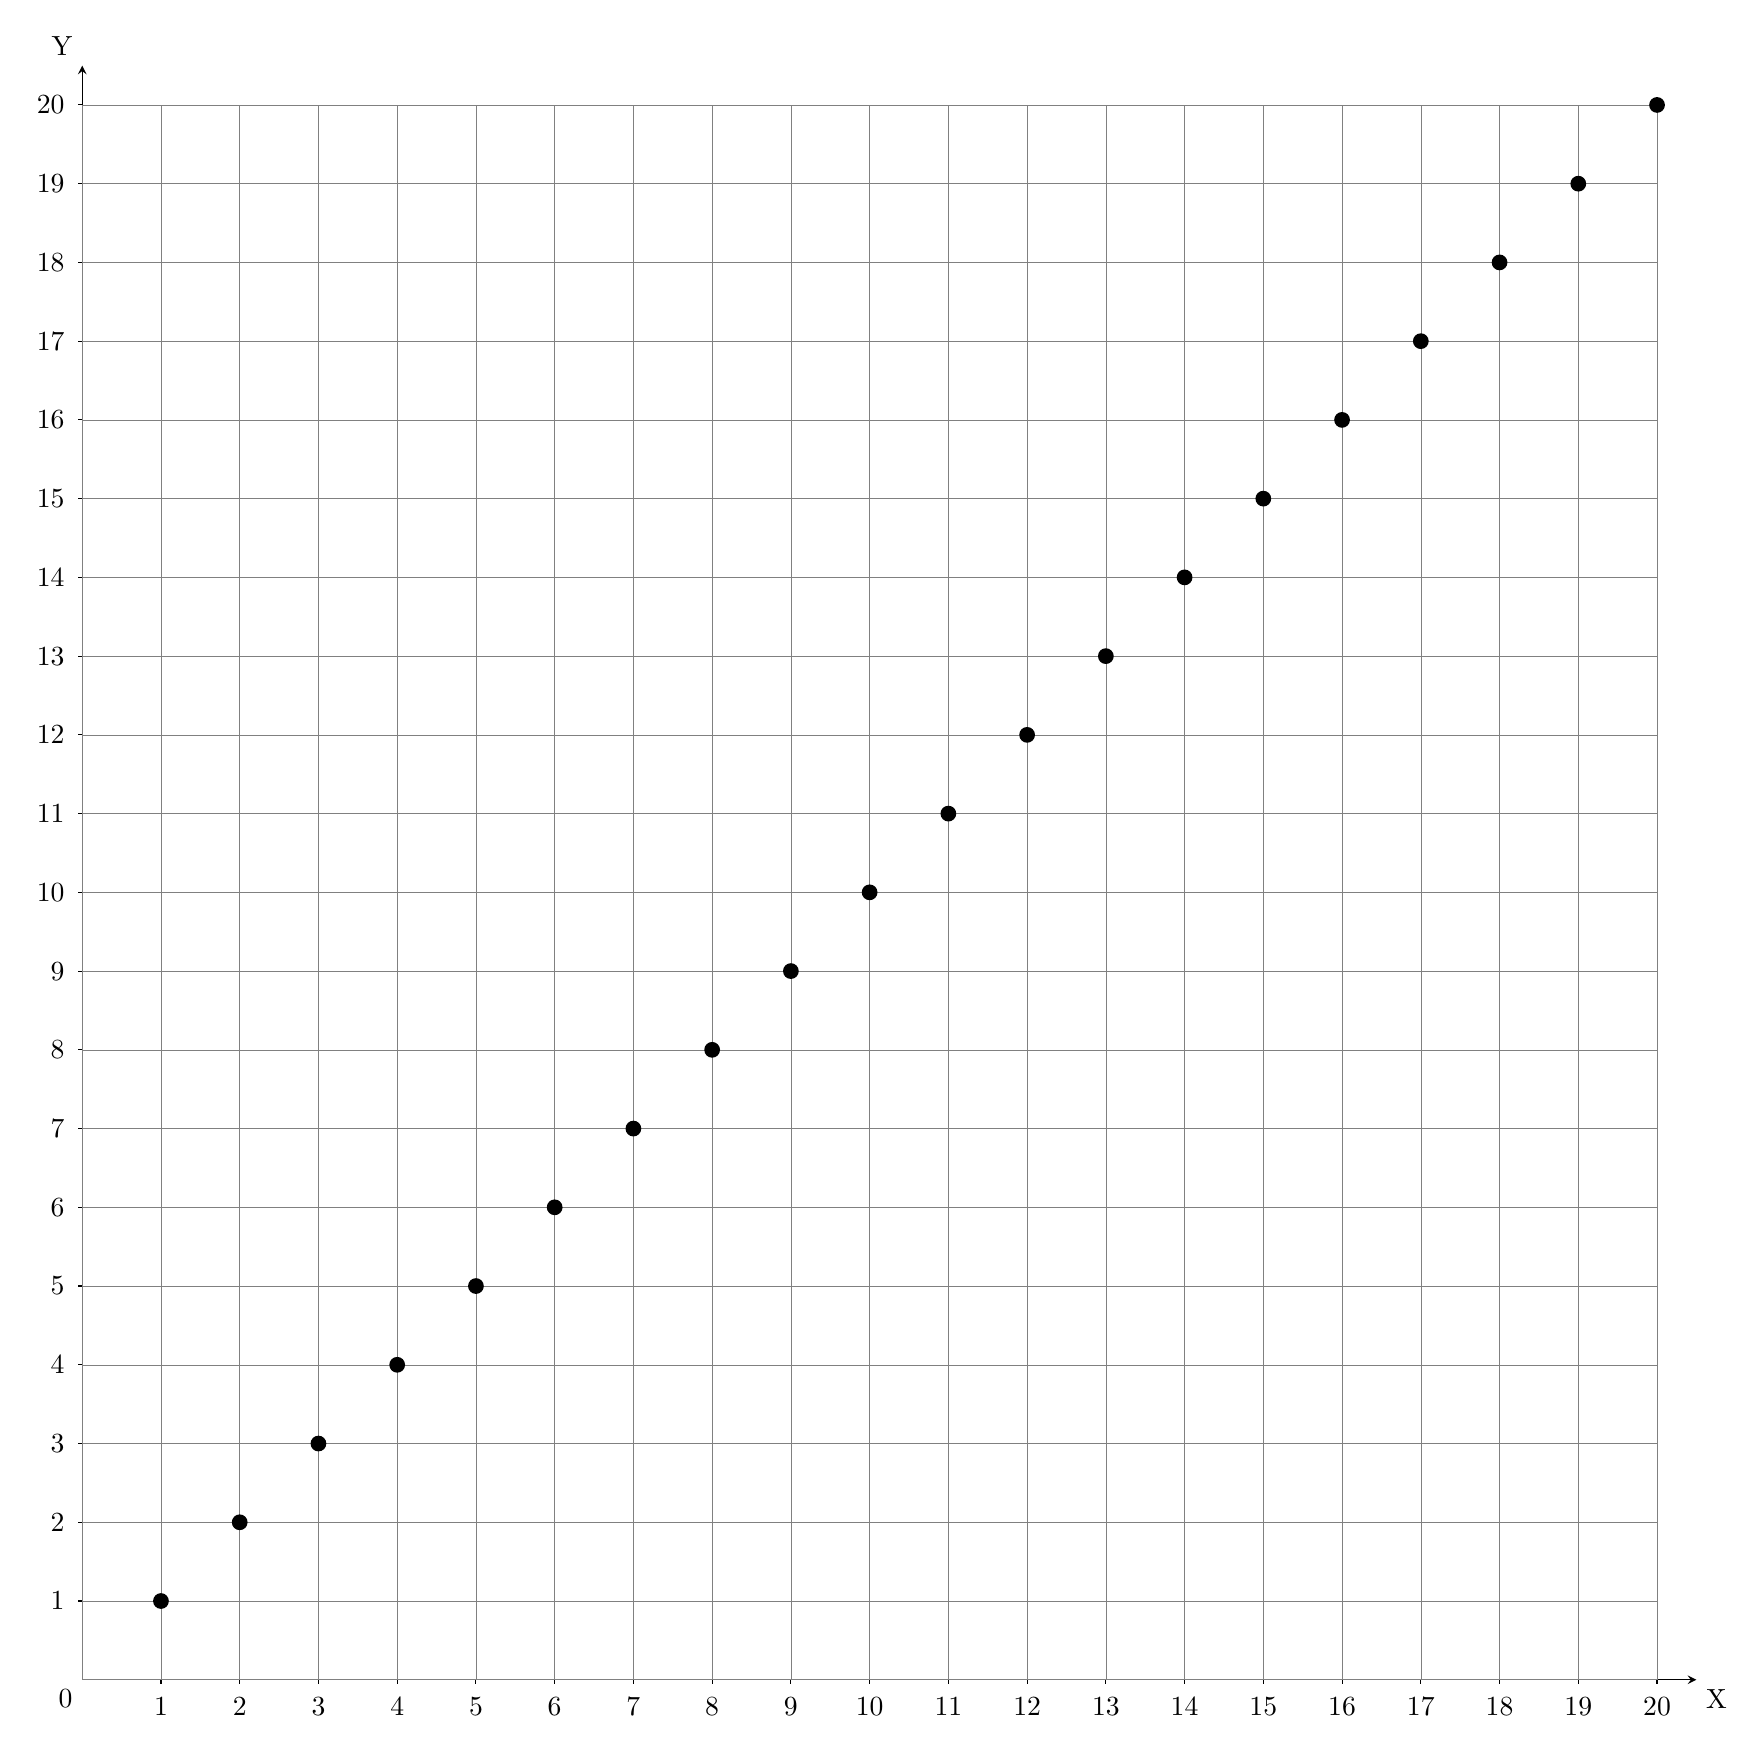
\begin{tikzpicture}
	\def\XMAX{20}
	\def\YMAX{20}
	%绘制横轴并在右下角标注X
	\draw [-stealth] (0,0) -- (0:\XMAX+0.5) node [below right] {X};
	%绘制纵轴并在右下角标注X
	\draw [-stealth] (0,0) -- (90:\YMAX+0.5) node [above left] {Y};	
	%标注原点
	\node at (0,0) [below left]  {0};
	%绘制辅助网格
	\draw [help lines, step=1] (0,0) grid (\XMAX,\YMAX);
	%绘制横轴的刻度线
	\foreach \i in {1,...,\XMAX} 
		\draw [black] (\i,-0.05) -- ++(90:0.05) node [below=1mm] {\i};
	%绘制纵轴的刻度线
	\foreach \i in {1,...,\YMAX} 
		\draw [black] (-0.05, \i) -- ++(0:0.05) node [left=1mm] {\i};
	
	%描点y=x
	\foreach \i in {1,...,\XMAX}
		\fill (\i,\i) circle(0.1) node [above] {};
		%\node [circle, fill] at (\i,\i) {};
\end{tikzpicture}    
\end{document}
